\begin{minipage}{0.35\textwidth}
    \begin{figure}[h]
    \centering
    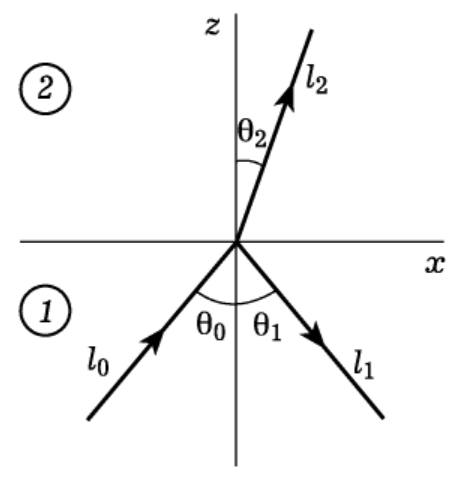
\includegraphics[width=1\textwidth]{images/brust.png}
    \caption{0 stands for a in-going wave, 1 stands for a transmitted wave, 2 stand for a reflected wave.}
    %\label{fig:}
\end{figure}
\end{minipage}
\hfill
\begin{minipage}{0.55\textwidth}
	 An incredible aspect describes the $\theta_p = \theta_0$ wich gives $\theta_0 + \theta_2 = \pi/2$.

	 With this and Snell's law we obtain:
	 \begin{equation}
	 	\tg \theta_p = \sqrt{\frac{\varepsilon_2}{\varepsilon_1}} = n.
	 \end{equation}
	 Where $\theta_p$ is the angle of polarization or \textit{Brewster's angle}.
\end{minipage}

